\documentclass[sheet=5]{exercise}
\setcounter{section}{20}
%
\begin{document}
%
\maketitle
%
\Remark{
	\section*{Hausaufgabe}
	\par Ab nächsten Montag sollten Sie beginnen Sich mit Ihrem
	Abschlussprojekt zu beschäftigen. Es gibt zwar noch Übungsblätter für
	Unentschlossene, aber die Erfahrung hat gezeigt, dass das Abschlussprojekt
	(welches ausschlaggebend für Ihre Endnote sein wird) sehr stark von einem
	frühen Beginn und den dadurch gewonnenen bereuten Tagen profitiert.
	\par Daher sollten Sie sich über das Wochenende Gedanken machen, was Ihnen
	Spaß machen könnte und als Projekt für Sie in Frage kommt.
}
%
\RequiredExercise{CSS Layout Grundlagen}
%
\par Verwenden Sie als Grundlage Aufgabe 6 von Blatt 2. Sollten Sie diese nicht
durchgeführt haben, so laden Sie sich die Lösung aus dem Internet herunter:
%
\begin{figure}[!h]
\centering
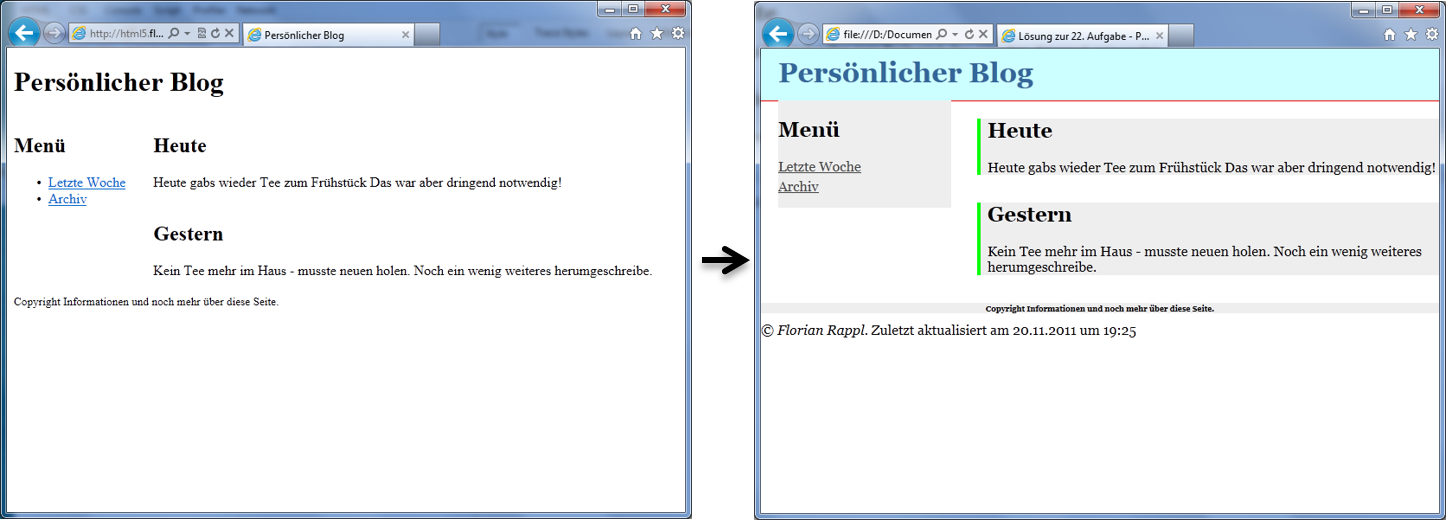
\includegraphics[width=1\textwidth]{Exercises/Figures/applycss.png}
\caption{Grau markiert sind die Bereiche der einzelnen Boxen}
\label{fig:applycss}
\end{figure}
%
\par Verwandeln Sie diese Seite durch CSS Code in das gezeigte Layout. Wichtig
sind hierbei folgende Details:
%
\begin{itemize}
\item
Die Seite soll die volle Fensterbreite ausnutzen.
\item
Der gesamte Text soll in der Schriftart \emph{Georgia} mit einer Schriftgröße
von \qty{12}{pt} angezeigt werden.
\item
Der Titel der Seite soll nach unten hin durch einen \qty{1}{px} Rahmen und
blaue Schrift abgegrenzt sein.
\item
Das Menü soll eine feste Breite von \qty{200}{px} und genau wie der Titel
\qty{10}{px} Abstand nach Links besitzen. Die Liste für das Menü soll keinen
Listenstil haben.
\item
Die Artikel sollen \qty{30}{px} Abstand zum Menü haben und einen linken Rahmen
haben. Jeder Artikel soll einen Abstand nach unten von 2em besitzen.
\item
Die Copyright-Information soll fett, in einer Schriftgröße von \qty{8}{pt} und
horizontal in der Mitte der Seite (unterhalb des gesamten Inhalts) angezeigt
werden. 
\item
Es dürfen keine fließenden Elemente, d.h.
%
\begin{lstlisting}
float: left; //oder
float: right;
\end{lstlisting}
%
verwendet werden.
\end{itemize}
\RequiredExercise{Zahlenraten mit Stil}
%
\par Die Grundlage für diese Aufgabe bietet Blatt 3 Aufgabe 14. Das Ziel
besteht darin dem Spiel ein aktuelles Design zu verpassen, welches absolut
platziert werden soll. Sollte Aufgabe 14 gelöscht oder nicht vorhanden sein,
so kann als Grundlage einfach die Musterlösung von der Webseite verwendet
werden.
%
\par Folgende Kriterien sollen vom Design erfüllt werden:
%
\begin{itemize}
\item
Jeder Container soll mittig auf der Seite platziert werden (und zwar bei jeder
Auflösung).
\item
Jeder Container soll eine Breite von \qty{600}{px} besitzen und eine Höhe von
\qty{400}{px}.
\item
Die Container sollen runde Ecken besitzen und einen Schatten werfen.
\item
Der Hintergrund der Seite soll einen ansprechenden (linearen) Farbverlauf
besitzen.
\item
Die Buttons sollen ein eigenes Design besitzen.
\item
Besonderer Text wie z.B. der Countdown sollen hervorgehoben werden (z.B.
größere Schrift, andere Farbe etc.).
\item
Der Inhalt der Container soll stimmig aussehen und den Platz im Container
ausnutzen.
\end{itemize}
%
\par Die Farbgestaltung sowie die Design-Feinheiten sind komplett Ihnen
überlassen. Denken Sie daran Ihr Design in verschiedenen Browsern zu testen
und Unterschiede weitesgehend zu erkennen und zu entfernen.
\RequiredExercise{Transformationen und Übergänge}
%
\par Erstellen Sie eine Seite, welche über fünf verschiedene \htag{div}-Boxen
verfügt. Jede Box soll dasselbe Grundlayout besitzen, welches aus einem
Rahmen, einer Hintergrundfarbe und einer bestimmten Größe besteht. Außerdem
sollen die Boxen einen festen Abstand voneinander besitzen.
%
\par Stellen Sie für alle Eigenschaften der Boxen ein Übergangsszenario von
zwei Sekunden Dauer ein. Jede Box soll außerdem beim Drüberfahren mit der Maus
(\emph{hover}) anders transformiert werden:
%
\begin{itemize}
\item
Die erste Box erhält eine Translation von \qty{50}{px} (horizontal) und
\qty{-20}{px} (vertikal).
\item
Die zweite Box erhält eine Translation um \qty{-15}{px}, \qty{30}{px} und eine
Rotation um \qty{90}{\degree}.
\item
Die dritte Box erhält eine Rotation um \qty{45}{\degree}.
\item
Die vierte Box erhält eine Verzerrung um \qty{50}{\degree} (vertikal) und eine
Rotation um \qty{50}{\degree}.
\item
Die fünfte Box erhält eine Verzerrung um \qty{25}{\degree} (horizontal), eine
Translation um \qty{50}{px} (vertikal) und eine Rotation um \qty{25}{\degree}.
\end{itemize}
%
\par Spielen Sie zum Abschluss noch mit einer zusätzlichen Transformation des
Containers der Boxen herum (vermutlich ist das in Ihrem Fall das
\htag{body}-Element). Was können Sie hierbei feststellen?
\Exercise{Ein bisschen SVG}
%
\par Ändern Sie das Zeichenprogramm von Blatt 4 so ab, dass es statt eines
\htag{canvas}-Elements SVG zeichnet. Sie können dies entweder in puren,
eigenständigem JavaScript oder durch Verwenden einer entsprechenden Bibliothek
wie RaphaëlJS lösen.
%
\par Erweitern Sie das Zeichenprogramm um folgende Möglichkeit: Nach dem
Hinzufügen eines Elementes soll dieses in eine \htag{select}-Liste aufgenommen
werden. Durch Klick auf einen entsprechenden Button soll das dort ausgewählte
Element aus dem Zeichenbereich entfernt werden.
\Exercise{Eine einfache Canvas Animation}
%
\par Entwerfen Sie eine HTML Seite, die ein \htag{canvas}-Element sowie drei
Buttons (Langsamer, Schneller, Abspielen / Pause) beinhaltet. Über den Button
Abspielen soll eine Animation (in Dauerschleife) gestartet werden. Beim
erneuten Klick auf den Button soll die Animation angehalten werden.
%
\par Gehen Sie am besten folgendermaßen vor:
%
\begin{itemize}
\item
Erstellen Sie eine \jfunc{drawCanvas}-Methode, die mit dem entsprechenden
Kontext Zeichnungen durchführt.
\item
Beim Klicken auf den Startbutton soll über \jfunc{setInterval} ein gepulster
Timer erstellt werden, der in regelmäßigen Abständen die
\jfunc{drawCanvas}-Methode ausführt.
\item
Beim erneuten Klick auf den Startbutton soll der Timer über
\jfunc{clearInterval} gelöscht werden.
\item
Schneller und Langsamer sollen nicht über die Pulsrate (d.h. Framerate)
kontrolliert werden, sondern über Eigenschaften, die in der
\jfunc{drawCanvas}-Methode verwendet werden (fett markiert).
\end{itemize}
%
\begin{figure}[!h]
\centering
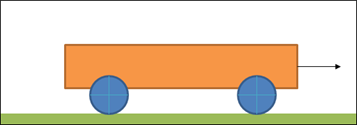
\includegraphics{Exercises/Figures/car.png}
\caption{Die zu zeichnenden Objekte}
\label{fig:car}
\end{figure}
%
\par Folgendes soll dabei gezeichnet werden:
%
\begin{itemize}
\item
Zwei Rechtecke (Orange und Grün)
\item
Zwei Kreise (Blau)
\item
Vier Linien in den Kreisen
\end{itemize}
%
\par Folgende Eigenschaften sollen animiert werden:
%
\begin{itemize}
\item
Die Position des orangen Rechtecks, der Kreise und der Linien (soll eine Fahrt
darstellen) über \jvar{dx}
\item
Der Winkel der Linien relativ zum Untergrund (soll bewegte Räder darstellen)
über \jvar{dalpha}
\end{itemize}
%
\par Sie können dies alles über Transformationen an den entsprechenden Stellen
erreichen. Für die Position sollten Sie \jfunc{translate} verwenden, für die
bewegten Räder \jfunc{rotate}. Vergessen Sie nicht, die Transformationen
entsprechend zurückzusetzen.

%
\end{document}